\documentclass[9pt,twocolumn,twoside]{pnas-new}
% Use the lineno option to display guide line numbers if required.
% Note that the use of elements such as single-column equations
% may affect the guide line number alignment.

\templatetype{pnasresearcharticle} % Choose template
% {pnasresearcharticle} = Template for a two-column research article
% {pnasmathematics} = Template for a one-column mathematics article
% {pnasinvited} = Template for a PNAS invited submission

\usepackage{pslatex}
\usepackage{amsfonts}
\usepackage{graphicx}
\usepackage{color}
\usepackage{todonotes}
\usepackage{dsfont}
\usepackage{array}
\usepackage{textcomp}
\usepackage{multirow}
\usepackage{subfig}

\newcommand{\mwu}[1]{{\color{green}{[mwu: #1]}}}


\title{Contextual flexibility in visual communication}

% Use letters for affiliations, numbers to show equal authorship (if applicable) and to indicate the corresponding author

\author[a,1]{Judith E. Fan}
\author[a]{Robert X.D. Hawkins}
\author[b]{Mike Wu}
\author[a,b]{Noah D. Goodman}

\affil[a]{Department of Psychology, Stanford University}
\affil[b]{Department of Computer Science, Stanford University}

% Please give the surname of the lead author for the running footer
\leadauthor{Fan}

\significancestatement{}

% Please include corresponding author, author contribution and author declaration information
\authorcontributions{Please provide details of author contributions here.}
\authordeclaration{Please declare any conflict of interest here.}
\correspondingauthor{\textsuperscript{1}To whom correspondence should be addressed. E-mail: jefan@stanford\@email.edu}

% Keywords are not mandatory, but authors are strongly encouraged to provide them. If provided, please include two to five keywords, separated by the pipe symbol, e.g:
\keywords{drawing $|$ deep learning $|$ pragmatics $|$ computational modeling $|$ Rational Speech Act framework}

\begin{abstract}

Visual modes of communication are ubiquitous in modern life --- from maps to data plots to political cartoons. Here we investigate drawing, the most basic form of visual communication. Communicative drawing poses a core challenge for theories of how vision and social cognition interact, requiring a detailed understanding of how sensory information and social context jointly determine what information is relevant to communicate. Participants (N=192) were paired in an online environment to play a drawing-based reference game. On each trial, both participants were shown the same four objects, but in different locations. The \textit{sketcher's} goal was to draw one of these objects --- the target --- so that the \textit{viewer} could pick it out from a set of distractor objects. There were two types of trials: \textit{close}, where objects belonged to the same category, and \textit{far}, where objects belonged to different categories. We found that people exploited information in common ground with their partner to efficiently communicate about the target: on far trials, sketchers achieved 99.7\% recognition accuracy while applying fewer strokes, using less ink, and spending less time (\textit{p}s$<$0.001) on their drawings than on close trials. We hypothesized that humans excel at this task by recruiting two core competencies: (1) \textbf{visual abstraction}, the capacity to perceive the correspondence between an object and a drawing of it; and (2) \textbf{social reasoning}, the ability to infer what information would help a viewer distinguish the target from distractors. We instantiated these competencies in a computational model that combines a multimodal convnet visual encoder with a Bayesian model of recursive social reasoning, and found that it fit the data well and outperformed lesioned variants of the model. Together, this work provides the first unified computational theory of how perception and social cognition support contextual flexibility in real-time visual communication.
\end{abstract}

\dates{This manuscript was compiled on \today}
\doi{\url{www.pnas.org/cgi/doi/10.1073/pnas.XXXXXXXXXX}}


\begin{document}

% Optional adjustment to line up main text (after abstract) of first page with line numbers, when using both lineno and twocolumn options.
% You should only change this length when you've finalised the article contents.
\verticaladjustment{-2pt}

\maketitle
\thispagestyle{firststyle}
\ifthenelse{\boolean{shortarticle}}{\ifthenelse{\boolean{singlecolumn}}{\abscontentformatted}{\abscontent}}{}

Communication is central to the success of our species: it allows us to learn from each other, coordinate our actions, and express otherwise hidden thoughts. People communicate in many ways, including spoken language and gesture. Critically, human communication goes beyond vocal production and manual signing: A watershed moment in the history of human communication was the invention of graphical representation, independently in Europe and Asia, about 30-60 thousand years ago \cite{hoffmann2018u,Aubert:2014jy}.

Graphical representation was transformative because it provided a means for people to encode their thoughts in a durable and shareable format. From ancient etchings on cave walls to modern digital displays, using graphical representations to communicate lies at the heart of key human innovations (e.g., mapmaking, data visualization), and forms the foundation for the cultural transmission of knowledge and higher-level reasoning. Drawing is a particularly important case study for understanding human visual communication. Drawn images predate symbolic writing systems \cite{clottes2008cave} are pervasive in many cultures \cite{gombrich1989story}, and are produced prolifically by children from an early age \cite{kellogg1969analyzing}.

%%%%%%%%%%%%%%%%%%%%

Communicative drawing poses a key challenge for understanding how

Successful visual communication by drawing inherently combines the activity of three such core systems: \textit{visual perception} --- the set of computations that transform raw visual inputs into semantically meaningful internal representations; \textit{social reasoning}

--- our robust capacity to evaluate other people's beliefs, intentions, and knowledge; determine action selection.

Drawing thus provides a natural domain to interrogate how visually-guided actions are constrained by high-level goals, including social communication, and likewise, how communicative behavior is constrained by our perceptual system.

A long-standing debate concerns the relative contribution of these systems for explaining how drawings derive their referential meaning. On the one hand, there is strong evidence that the perceptual system is sufficient to explain how people are able to perceive the correspondence between drawings and real-world objects, suggesting that this ability can arise from the same general-purpose neural architecture evolved to handle natural visual inputs
\cite{fan2015common, yamins2014performance}. On the other hand, several influential theorists have argued that socially-mediated experience with pictorial representations is always necessary to be able to extract semantic content from drawings \cite{goodman1976languages,gombrich1989story}.

How can these two opposing perspectives on the basis for fluency with graphical representations be reconciled? And how does such variation in visual communication behavior, ranging from the depictive to the symbolic, arise from the same cognitive architecture? Here we propose a unified theoretical framework for understanding how such variation naturally arises from variation in context, affecting how perception and social inference are combined to generate communicative actions.


Here we propose an integrated computational model of visual communication that combines high-performing models of sensory representation from deep learning with insights from Bayesian cognitive models of social reasoning in language.

This  into the core computations that connect perception, action, and social cognition to support visual communication.

%%%%%%%%%%%%%%%%%%%%

The goal of this paper is to evaluate the hypothesis that contextual flexibility in human visual communication can be captured by combining constraints from perception and pragmatic reasoning.

Specifically, are \emph{pragmatic visual communicators} who proactively account for their viewer's expectations and take advantage of shared knowledge to be informative
\cite{wilson1986relevance,goodman2016pragmatic}
while also being parsimonious \cite{zipf1936psycho}.




\section*{Results}

\subsection*{Behavioral task performance}

%%%%% List of results figures
%% Figure 1: Task Display & Design & example drawings [first draft ready]
%% Figure 2: Communication Game Task Performance & Recognition Task Performance
%% Figure 3: Model schematic
%% Figure 4: Model comparison & evaluation (absolute performance) -- human+RSA (2 production x 2 pragmatics = 4 bars) + VGG+RSA (2 production x 2 pragmatics x 3 perception = 12 bars)

%% Supplemental 1: Perceptual similarity -- maybe confusion matrix
%% Supplemental 2: Param posteriors
%% Supplemental 3: Error analysis for each lesioned versions

\begin{figure*}[htbp]
\centering
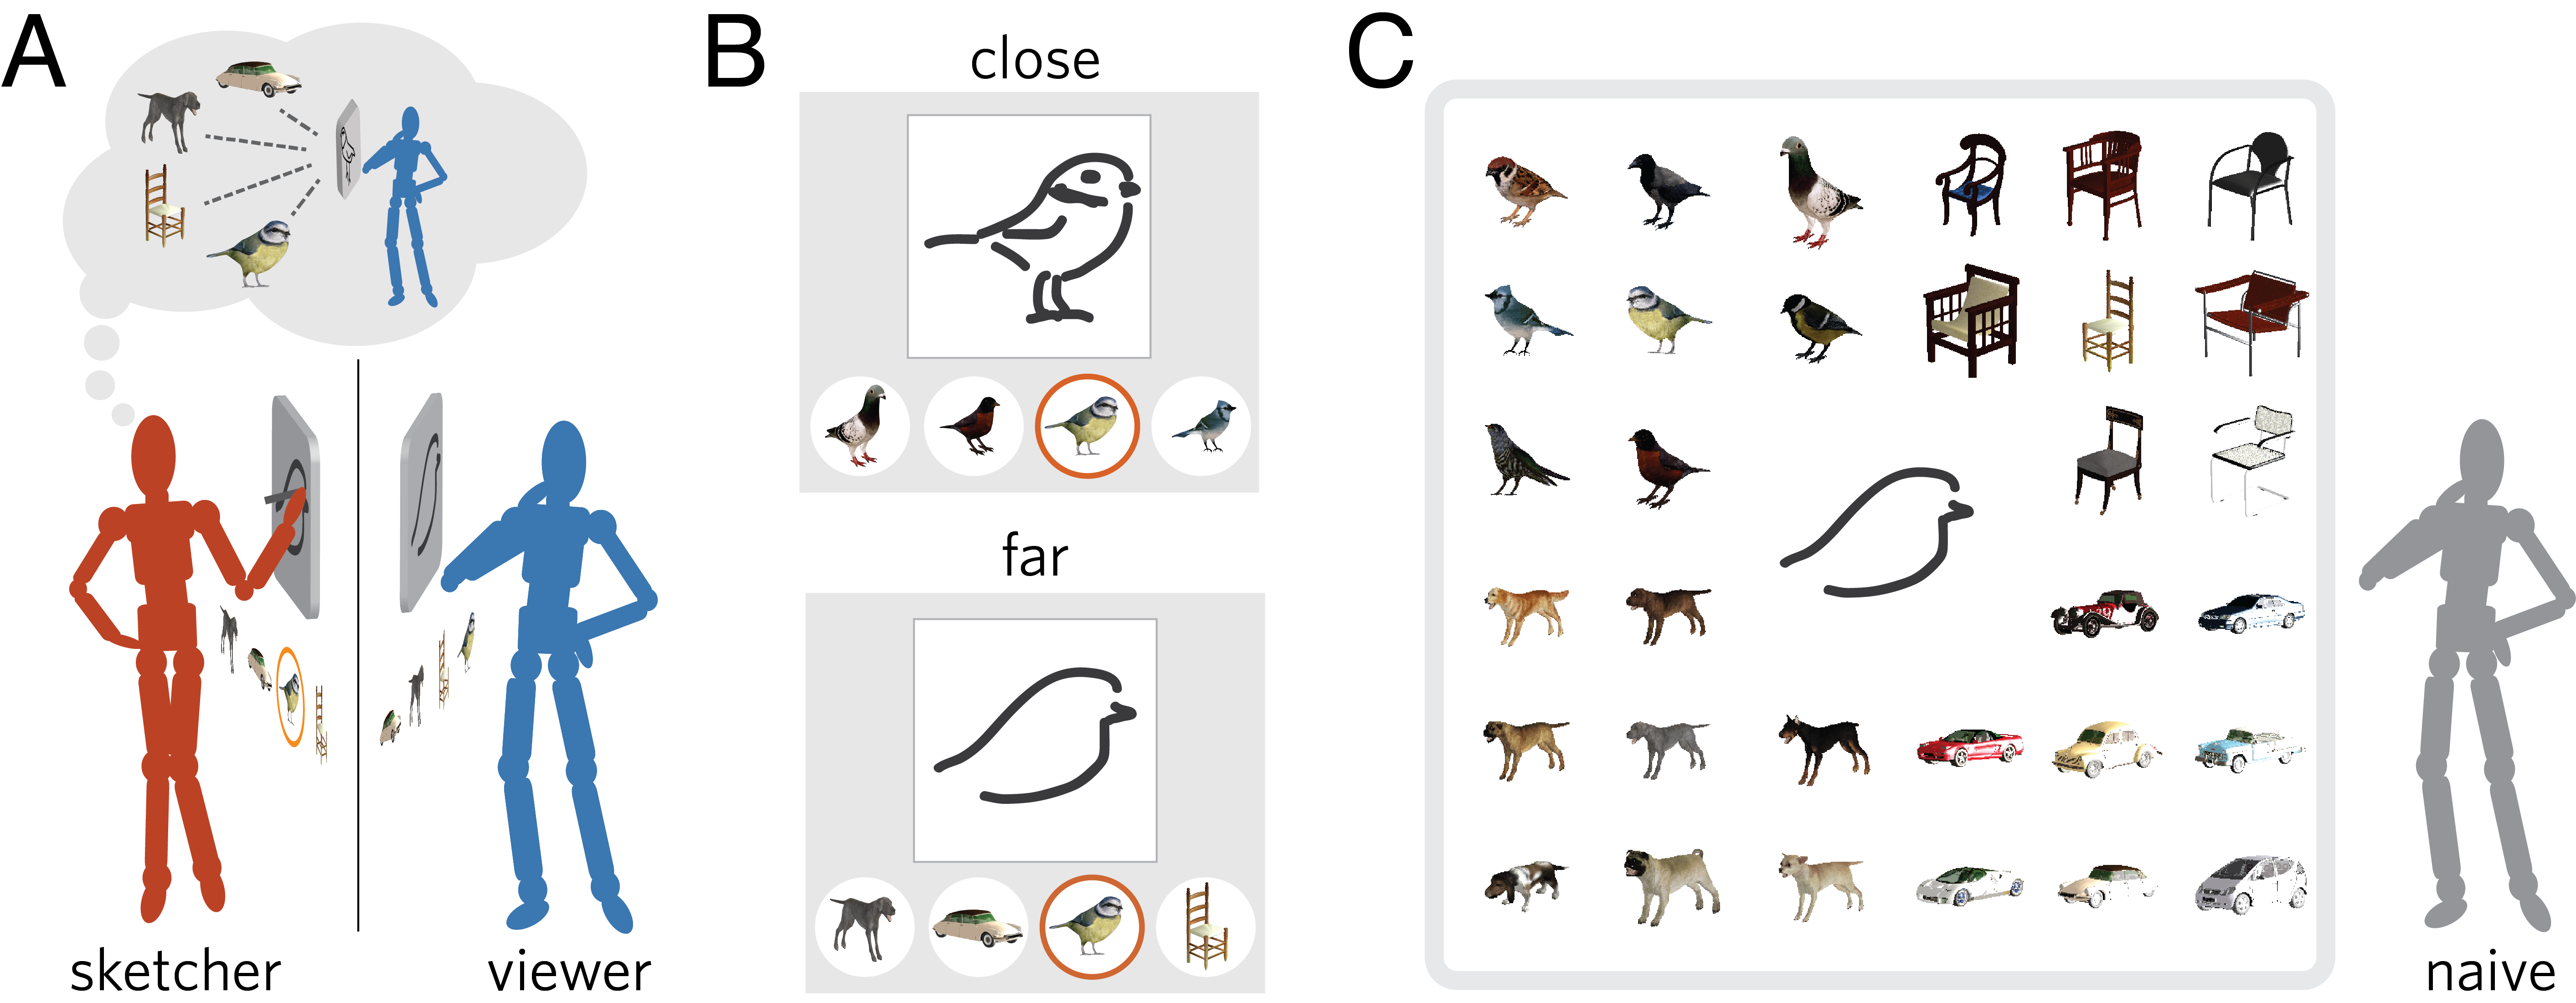
\includegraphics[width=0.95\textwidth]{figures/1_task_display.pdf}
\caption{(A) Communication task. (B) Context manipulation. (C) Recognition task.}
\label{task_display}
\end{figure*}


We hypothesized that sketchers aim to be informative yet parsimonious in communicating about the target object in context.

We evaluated several predictions that this hypothesis makes:

first, that sketchers are generally successful at conveying the identity of the target to viewers in both close and far contexts.

second, that sketchers will modulate the level of detail in their drawings according to the similarity of the alternatives under consideration by the viewer.

If sketchers aim to make their sketches informative without being too costly to produce, they will modulate the level of detail in their drawings according to the set of alternatives under consideration by the viewer.

\begin{figure*}[htbp]
\centering
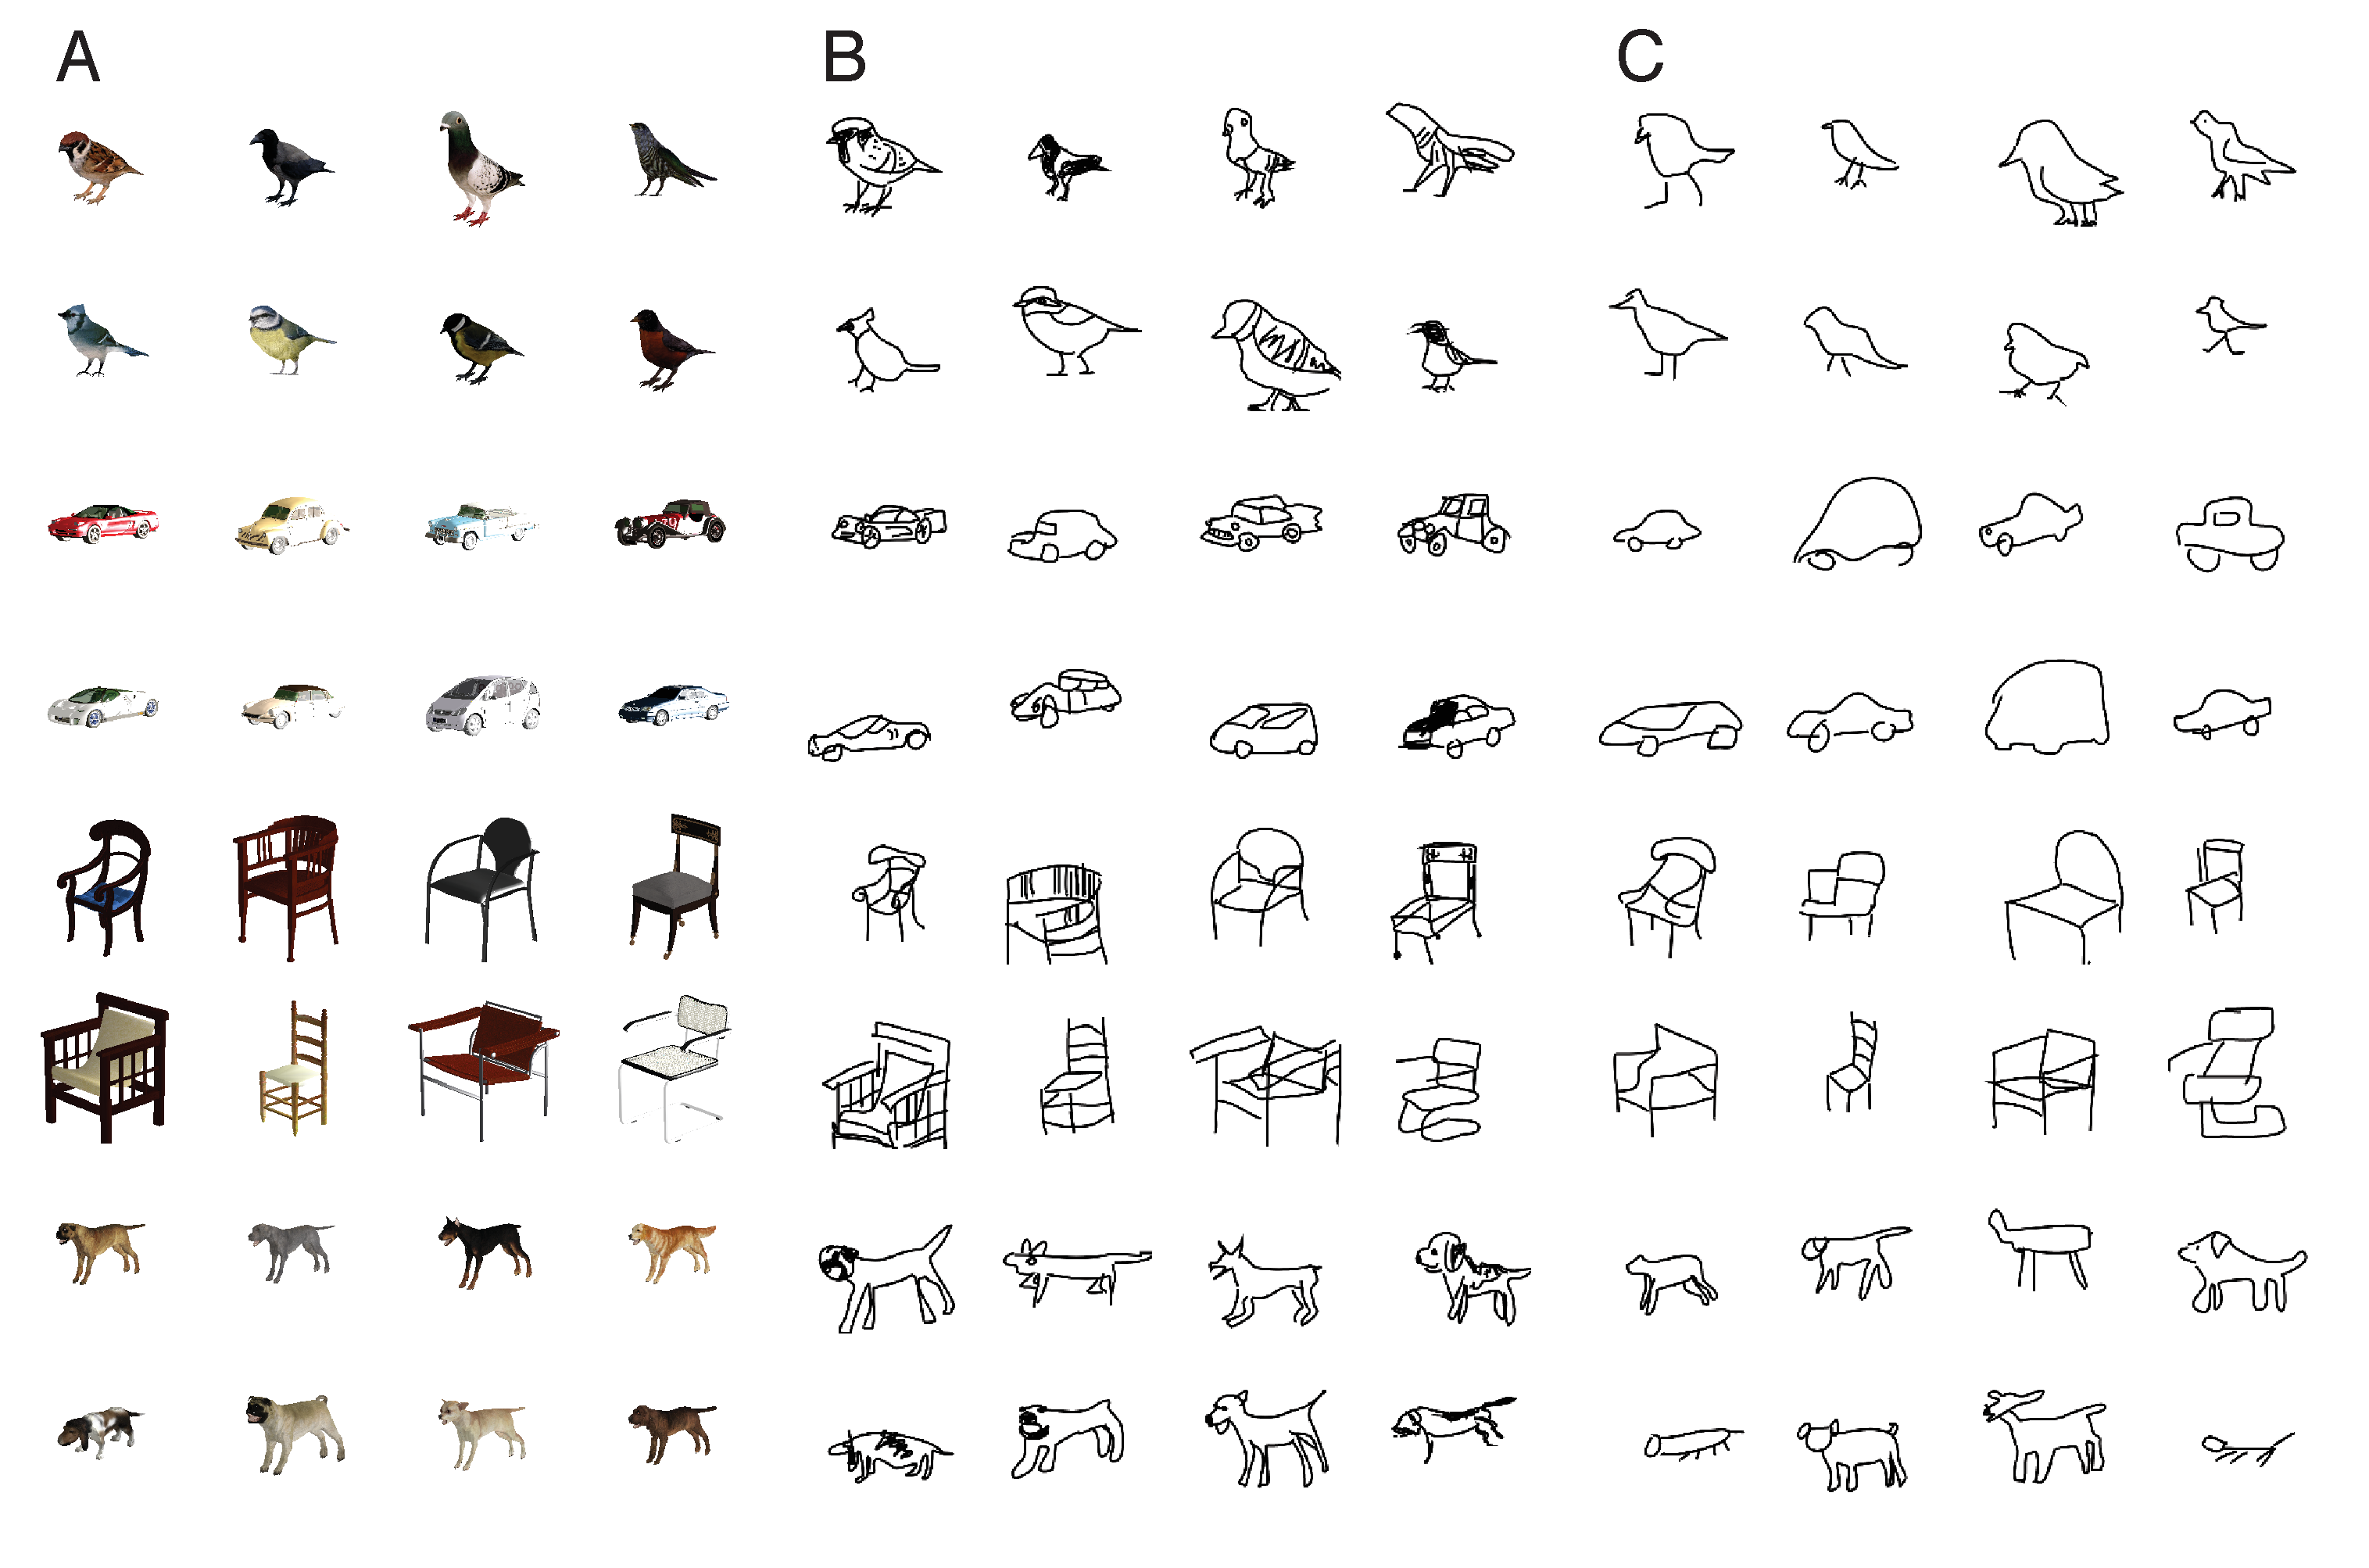
\includegraphics[width=0.95\textwidth]{figures/2_sketch_gallery.pdf}
\caption{(A) Object stimuli. (B) Example sketches produced in close condition. (C) Example skeches produced in far condition.}
\label{sketch_gallery}
\end{figure*}


For instance, in the \textit{close} condition where the target and distractors belong to the same basic-level category, sketchers should make detailed drawings to highlight fine-grained distinctions, even though this requires including additional detail. By contrast, in the \textit{far} condition where the target and distractors belong to different basic-level categories, the sketcher can afford to produce simpler drawings by omitting excess detail.

Consistent with this prediction, we found that sketchers applied fewer strokes (close = 8.03, far = 13.5, \textit{p} $<$ 0.001), used less ink (measured by proportion of the canvas marked: close = 0.054, far = 0.042, \textit{p} $<$ 0.001) and spent less time (close = 30.3s, far = 13.7s, \textit{p} $<$ 0.001) to make their drawings in the far condition than in the close condition.

Despite the relative sparsity of drawings produced on far trials, viewers were close to ceiling on inferring the target (99.7\%). Performance was also high on close trials (87.7\%), even though this required that people discriminate the correspondence between a sketch and its referent in the context of highly similar distractors.

We hypothesized that the context manipulation in the communication experiment systematically affected the high-level perceptual content in participants' sketches, resulting in Far sketches that were highly informative about the target \textit{in context} yet less recognizable (i.e., worse match to the target object) than Close sketches \textit{out of context}.

In other words, we predicted that the decreased effort expended by participants on Far trials reduced the absolute perceptual similarity between sketches and the target. The goal of this experiment was to validate this assumption and to provide independent training data to train a shallow adaptor network to merge photorealistic images and sketches into a common latent space, from which perceptual similarity can be easily read out.


\begin{figure*}[htbp]
\centering
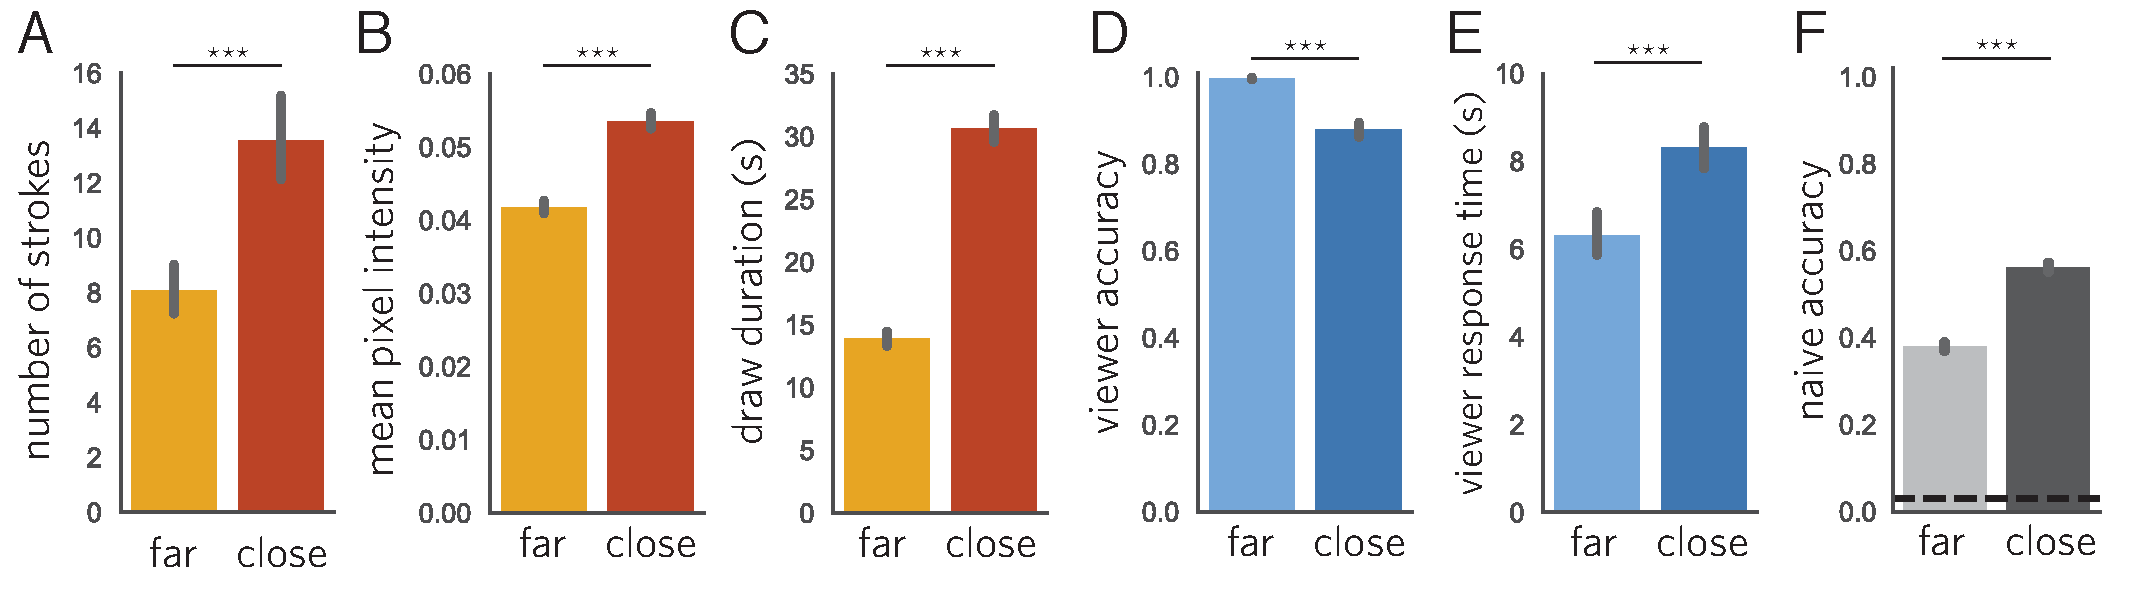
\includegraphics[width=0.95\textwidth]{figures/3_behavioral_performance.pdf}
\caption{(A-C) Sketchers used fewer strokes, less ink, and spent less time producing sketches in the far condition, relative to the close condition. (D-E) Viewers were at ceiling accuracy in identifying the target in the far condition, and were highly accurate in the close condition. (F) Naive matcher participants were more accurate for close sketches than far sketches.}
\label{task_performance}
\end{figure*}


%%% recognition experiments
%% report close vs. far Accuracy

Consistent with our prediction, we found that Close sketches were matched with their corresponding object rendering much more frequently than Far sketches were (Close: 54.2\%; Far: 37.5\%; $Z$=14.1, $p$<0.001), although both were successfully matched at rates far exceeding chance ($p$s < 0.001).

%% report variation in different categories

%% report confusion matrix results: diagonal vs. off-diagonal block vs. rest of the matrix results.

We further hypothesized that the particular way in which Far sketches would differ perceptually from Close sketches was that Far sketches would be more confusable with other objects from the same basic-level category, while still being highly recognizable as a representation of the corresponding basic-level category.

We measured this by comparing the within-category confusion rate to the overall confusion rate for Close and Far sketches, and found that XXX.

\subsection*{Modeling pragmatics and cost}

%% describe the full sketcher model
To make fine-grained quantitative predictions and conduct a rigorous comparison, we formalized our hypotheses as a series of computational models. Our full sketching model integrates three key components: \emph{production}, \emph{pragmatics}, and \emph{perception} (see \emph{Materials and Methods}; Eq. 2-4 and Fig. \ref{fig:modelSchematic}). \emph{Production} determines whether or not the agent accounts for the relative cost of producing drawings with more strokes. \emph{Pragmatics} captures the sketcher's reasoning about how a viewer will make decisions in context. \emph{Perception} determines the encoding model used by the agent to determine the literal similarity between a drawing and object. Intuitively, putting these components together has the effect of biasing the model to depict properties of the target object that perceptually distinguish it from the distractors, while also preferring sketches that are less costly to produce, i.e., requiring fewer strokes or less ink. We conduct a set of comparisons against lesioned variants to test the role played by each component.

%% report RSA modeling results using human perceptual measurements directly to compute informativity
%% prag with cost, prag no cost, no prag cost, no prag no cost
We begin with production and pragmatics. Lesioning the production component simply requires setting the parameter weighting the \emph{cost} term of our speaker's utility to zero, such that all sketches are equally easy to produce. For the pragmatic component, we compare a \emph{social sketcher}, which takes context into account, against an \emph{asocial sketcher} that simply aims to make a sketch with high absolute perceptual similarity to the target, ignoring context. To define our social sketcher, we generalize the Rational Speech Act (RSA) framework from the linguistic domain, where it has captured language use as a process of recursive social reasoning \cite{stuff}. By reasoning about a viewer who normalizes perceptual similarity across objects in context, a social sketcher is able to choose sketches that are \emph{informative}, or that apply to the target relatively better than distractors. For example, in a context only containing birds, a generic outline of a bird would not be very informative, even if it has high absolute similarity to the target, because it also resembles the distractors. Because both absolute and relative similarity may influence a sketcher's decision, we introduced a parameter $w_p \in [0,1]$ that interpolates between the two values. We conducted a Bayesian Data Analysis, plugging in the similarity function directly estimated from empirical human ratings in the matching task. We found that the social speaker was strongly preferred over the asocial speaker ($BF = XX; w_p = YY$, 95\% credible interval $= [X, Y]$) and the model including a cost term was strongly preferred over a cost-free variant ($BF = XX; w_c = YY$, 95\% credible interval $=[X, Y]$; see Fig. \ref{fig:model_results}A).

\subsection*{Modeling perception}
%% report RSA modeling results, where we apply the same 2 pragmatics (prag vs. no prag) x 2 production (cost vs. no cost) x 4 perception (pool1, conv42, fc6, human) comparison categories
Next, to test the influence of perceptual representations, we compared our empirically measured similarity values with three alternative similarity functions lightly adapted from different layers of a convolutional neural network (see \emph{Materials and Methods}, Eq. 1). Critically, because these are \emph{encoding} models that take raw visual input, they can generalize to entirely novel sketches. One of the most striking aspects of visual communication is the human ability to recognize an object from a handful of strokes, even though the respective images have little to no overlap in low-level visual features. Motivated by prior work \cite{fan2015common}, we hypothesized that performance in visual communication would improve as we ascend the layers of a visual encoding model.  We augmented a high-performing deep convolutional neural network architecture with a smaller \emph{adaptor} network that was trained on the data from our matching task and learned a common feature representation for drawings and photos. We conducted another Bayesian Data Analysis comparing feature vectors adapted from \emph{pool1}, \emph{conv42}, and \emph{fc6}, respectively, as our raw similarity function. We found that the sketcher adapted from the later layer of \emph{fc6} performed better than the mid-layer of \emph{conv42} ($BF= XX$, which in turn performed better than \emph{pool1} ($BF = XX$; see Fig. \ref{fig:model_results}B).

\begin{figure*}[htbp]
\centering
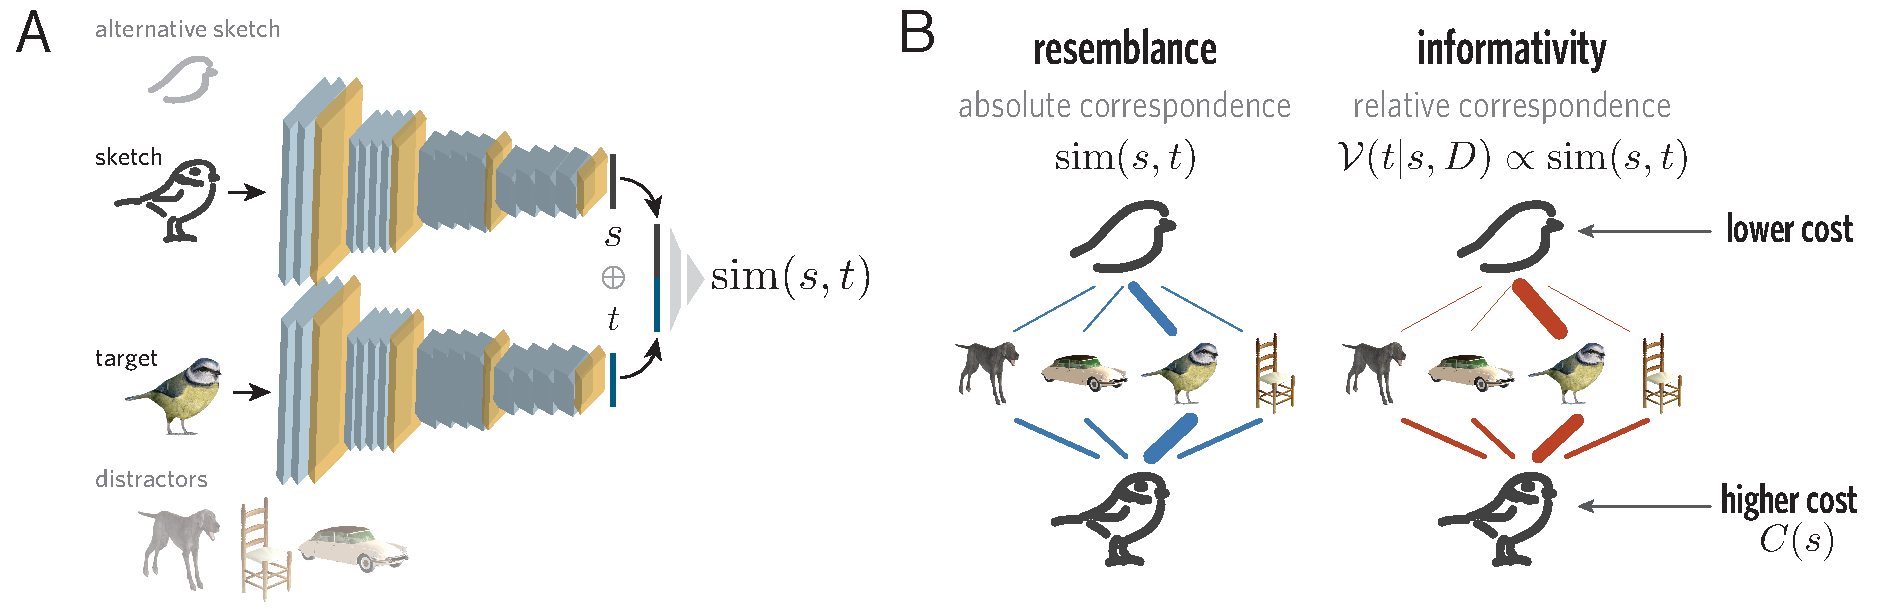
\includegraphics[width=0.95\textwidth]{figures/4_model_schematic.pdf}
\caption{(A) Architecture of visual encoder model for sketches and object renderings. Consists of pre-trained deep convolutional neural network (VGG-19) and shallow nonlinear ``adaptor'' neural network to evaluate sketch-object similarity. Takes a sketch and object image as input, and outputs a similarity score reflecting how well the sketch resembles the object. Adaptor was trained on a subset of our dataset, and evaluated on held-out sketches. (B) Sketch-object similarity computed for each object in context and each sketch in the test set. To determine the relative informativity of each sketch, the similarity scores between this sketch and all four objects were softmax normalized. The cost of each sketch was assumed to vary with the amount of time taken to produce it.}
\label{task_performance}
\end{figure*}


%% report generalization performance of visual adaptor on the appropriate splits?

\subsection*{Evaluating model performance}
Having established the need for all three components, we proceed to


\subsubsection*{Code availability} The code for the analyses presented in this article is publicly available in a Github repository at: XX.

\subsubsection*{Data availability} The data presented in this article are publicly available at this URL: XX.
ras
\subsection*{Supporting Information (SI)}

% The main text of the paper must stand on its own without the SI. Refer to SI in the manuscript at an appropriate point in the text. Number supporting figures and tables starting with S1, S2, etc. Authors are limited to no more than 10 SI files, not including movie files. Authors who place detailed materials and methods in SI must provide sufficient detail in the main text methods to enable a reader to follow the logic of the procedures and results and also must reference the online methods. If a paper is fundamentally a study of a new method or technique, then the methods must be described completely in the main text. Because PNAS edits SI and composes it into a single PDF, authors must provide the following file formats only.

\matmethods{

\subsection*{Communication experiment: Manipulation of context in sketch-based reference game}

\subsubsection*{Participants}

A total of 192 unique participants, who were recruited via Amazon Mechanical Turk (AMT) and grouped into pairs, completed the experiment. They were provided a base compensation of \$X.XX for participation and earned a \$X.XX bonus for each correct trial. In this and subsequent behavioral experiments, participants provided informed consent in accordance with the Stanford IRB.

\subsubsection*{Stimuli}

Stimuli were 32 3D mesh models of objects belonging to 4 categories (i.e., birds, chairs, cars, dogs), containing eight objects each. 40 color images of each object were produced by rendering it from a 10$^{\circ}$ viewing angle (i.e., slightly above) at a fixed distance on a gray background, each rotated by an additional 9$^{\circ}$ about the vertical axis.

\subsubsection*{Task}

Drawings were collected in the context of an online, sketching-based reference game (``Guess My Sketch!''). The game involved two players: a \textit{sketcher} who aims to help a \textit{viewer} pick out a target object from a set of distractor objects by representing it in a sketch. On each trial, both participants were shown an array of the same four objects; however, the positions of these objects were randomized for each participant. On each trial, one of the four objects was highlighted on the sketcher's screen to designate it as the target.

Sketchers drew using black ink on digital canvas (pen width = 5 pixels; 300 x 300 pixels) embedded in a web browser window using Paper.js (http://paperjs.org/). Participants drew using the mouse cursor, and were not able to delete previous strokes. Each stroke of which was rendered on the viewer's screen immediately upon the completion of each stroke. There were no restrictions on how long participants could take to make their drawings. After clicking a submit button, the viewer guessed the identity of the drawn object by clicking one of the four objects in the array. Otherwise, the viewer had no other means of communicating with the sketcher. Both participants received immediate task-related feedback: the sketcher learned which object the viewer had clicked, and the viewer learned the identity of the target. Both participants earned bonus points for each correct response.

For each pair, objects were grouped into eight quartets: Four of these quartets contained objects from the same category (``close''); the other four of these quartets contained objects from different categories (``far'' condition). Each quartet was presented four times, such that each object in the quartet served as the target exactly once. The assignment of objects to quartet and condition was randomized across pairs.

\subsection*{Recognition experiment: Measuring perceptual similarity between sketches and objects}

\subsubsection*{Participants}

A total of 112 participants were recruited via Amazon Mechanical Turk (AMT). They were provided a base compensation of \$1.00 for their participation, and earned an additional \$0.01 bonus for each correct response.

\subsubsection*{Task}

On each trial, participants were presented with a randomly selected sketch collected in the sketch-based reference game, surrounded by a grid containing the 32 objects from that experiment. Their goal was to select the object in the grid that best matched the sketch. Participants were instructed to prioritize accuracy over speed. A small proportion of outlier trials that were either too fast (response latency <1000ms) or too slow (>20s) were filtered from the dataset; we reasoned that behavior on such trials was likely to be noisier and not comparable to that on the remainder of trials. The removal of these outlier trials did not have a substantial impact on the pattern of recognition behavior. In order to mitigate the possibility that participants could adjust their matching strategy according to any particular sketcher's style, each session was populated with 64 sketches sampled randomly from different reference games. Participants were provided with binary feedback about the correctness of their response on each trial via a bonus counter that incremented by 1 point for each correct identification, but did not change for incorrect trials.

% VERIFY THIS: Participants were permitted to complete multiple sessions of this task, but were prevented from providing identification judgments for the same sketch twice, or for sketches they themselves had produced or viewed (on the rare occasion that this participant had also participated in the reference game experiment).

\subsection*{Computational modeling}


\subsubsection*{Visual encoder module}

Features were extracted using VGG-19 \cite{simonyan2014very}, a high-performing deep convolutional neural network model architecture that had been pretrained to categorize objects on the Imagenet database, which contains millions of photographs from hundreds of object categories \cite{deng2009imagenet}. Despite the fact that drawings are highly abstracted away from natural visual inputs, prior work has shown a striking isomorphism in the similarity structure \cite{kriegeskorte2008matching} of object categories in drawings and photos at higher layers in these models \cite{fan2015common}, without any additional training.

While these models excel at (and were indeed optimized for) categorization of objects, two additional competencies are required to succeed at the visual communication task described above. First, an observer must be able to represent fine-grained relationships between different images of objects from the same category; second, this observer must also be able to discern image-level correspondences between drawings and photos of the same object. In order to better approximate the granularity with which human observers can distinguish different images, we augment VGG19 with a smaller \textit{adaptor} network that learns a common feature representation for drawings and photos. This approach has been successfully used in prior work to better predict human semantic categorization judgments \cite[]{peterson2016adapting}, and to improve sketch-based image retrieval \cite[]{sangkloy2016sketchy}.

We explore adapting features from three different layers of VGG-19: the first max pooling layer (vgg-early), the tenth convolutional layer (vgg-mid), and the first fully connected layer (vgg-high), respectively representing low, medium, and high level visual abstraction. As such, we design three different encoder models, intentionally keeping them lightweight and comparable in number of parameters (Table~\ref{table:parameters}). We respectively refer to these as \textit{adaptor-early}, \textit{adaptor-mid}, and \textit{adaptor-high}. Below, we detail the architecture and hyperparameter choices:

Adaptor-high is composed of a linear layer from 8192 to 512, followed by a swish nonlinearity \cite[]{ramachandran2018searching} and dropout, then a linear layer from 512 to 1. Each vgg-high feature has 4096 dimensions. A photo and sketch feature is first concatenated to form a vector of size 8192, then passed to adaptor-high. Empirically, we find the ability of the model to fit the data robust to the choice of nonlinearity and hidden dimensionality.

\begin{table}
\centering
\begin{tabular}{| l | c |}
\hline
Model & Parameters \\
\hline
\hline
adaptor-early & 4195329 \\
\hline
adaptor-mid & 526881 \\
\hline
adaptor-high & 33409 \\
\hline
\end{tabular}
\caption{Number of parameters in the visual encoder modules.}
\label{table:parameters}
\end{table}

Similarly, adaptor-mid consists of a linear layer of 1024 to 512, swish, dropout, then a linear layer from 512 to 1. Since vgg-mid features are three dimensional (512 by 28 by 28), we first flatten the input into a one dimensional vector of size 512 using a weighted linear combination $\sum_{i=1}^{28}\sum_{j=1}^{28} w_{ij} * x_{ij}$, where $x_{ij}$ represents a cross-section from vgg-mid. The parameters $\{w_{ij}|1\leq i,j \leq 28\}$ are learned along with the parameters of adaptor-mid. Intuitively, this is akin to attention over the spatial features of vgg-mid. We separately attend over photo and sketch spatial features, creating two vectors of size 512, then concatenate prior to adaptor-mid.

Finally, adaptor-low is almost identical to adaptor-mid, except each feature is of size 64 by 112 by 112. Explicitly, this network starts with a linear layer of 4096 to 64, swish, dropout, then a linear layer form 512 to 1. Due to the input size, each attention module has 12,544 learnable weights.

%% adaptor training procedure
We now describe the training procedure for each visual encoder. The sketch dataset is split into training, validation, and test sets in a 80\%, 10\%, and 10\% ratio. This division is performed based on context, which is defined as the set of the target and distractor images (each trial consists of 3 distractor images and 1 target). Doing so, the contexts of training examples will not overlap with the contexts of either validation or test examples. Given a photo and a sketch, the adaptor network outputs a single real number, which we use as a similarity measure. We construct of similarity vector of size 32 between a sketch and each photo in the domain (32 total), and apply a softmax on top to induce a probability distribution over photos. To fit network parameters, we optimize via stochastic gradient descent on a cross entropy loss between the induced distribution and a distribution of average human choices (\mwu{@judy add more details about how we get labels}). Specifically we use Adam \cite[]{kingma2014adam} with a learning rate of 1e-4 with a minibatch size of 10 for 100 epochs. As a property of the input domain, the gradients with respect to adaptor parameters are by default, very small. While increasing the learning rate may lead to unstable optimization, we find that multiplying the loss by a large constant $C$ is necessary to sufficiently optimize the objective for good test performance. In practice, $C = 10000$. Post-training, we use the model with the best loss on a held-out validation set. For each photo and sketch pair in the test set, we calculate the similarity score as input to a social reasoning module.

\subsubsection*{Social reasoning and decision-making module}

We formalize a sketcher, $\mathcal{S}$ as a decision-theoretic agent who produces sketches, $s$, by (soft)-maximizing their utility function, $U$, given a particular object referent, $o$:

\begin{equation}
\mathcal{S}(s|o) \propto \exp\{{U(s,o)\}}
\end{equation}

The utility function of our pragmatic sketcher, $U_{S_1}$,  trades off the extent to which the sketch is informative to the viewer, $\mathcal{V}$, and the cost of producing the sketch, $C(s)$. This notion of informativity is defined by the (natural log) probability that a viewer would select the true object referent given the drawing and current context.

\begin{equation} \label{sketcher_utility}
U_{S_1}(s, o) = w_p \ln \mathcal{V}(o|s) - w_c C(s)
\end{equation}
where $w_p$ and $w_c$ are latent parameters weighting the influences of the sketch's perceptual properties and cost, respectively.

The viewer ($\mathcal{V}$) is assumed to choose among potential objects in context proportional to their perceptual similarity vis-a-vis the drawing.

\begin{equation} \label{literal_viewer_score}
\mathcal{V}(o|s) \propto \exp\{\alpha \cdot \textrm{sim(s, o)}\}
\end{equation}
where $\alpha$ is a scaling parameter determining the assumed optimality of the listener's decision policy: as $\alpha \rightarrow \infty$, the listener increasingly chooses the object with maximum perceptual similarity to the sketch.

We also consider a literal sketcher $S_0$ who does not reason about a viewer in context, but tries to directly maximize the perceptual similarity of their sketch to the target, thus we use $\textrm{sim}(s, o)$ instead of informativity to $\mathcal{V}(o|s)$ in their perceptual term. To infer the effect of pragmatics, we infer the mixture of these speakers that best fits the data. We introduce an additional parameter $w_{prag}$ that interpolates between their utilities: $$f(s,o) = w_{prag}\ln \mathcal{V}(o | s) + (1-w_{prag}) \textrm{sim}(s,o)$$ After algebraically simplifying, the full utility is :

\begin{equation}
U(s,o) =  w_p \cdot  f(s,o) - w_c \cdot C(s)
\end{equation}

To compute perceptual similarity, we extract a feature vector representation from each of the target and distractor objects using the selected fixed visual encoder, and compute the (logged) distances between each of these vectors and the potential sketches.
}

\showmatmethods % Display the Materials and Methods section

\acknow{Thanks to XX, XX, XX for helpful comments and discussion.}

\showacknow{} % Display the acknowledgments section

% \pnasbreak splits and balances the columns before the references.
% Uncomment \pnasbreak to view the references in the PNAS-style
% If you see unexpected formatting errors, try commenting out \pnasbreak
% as it can run into problems with floats and footnotes on the final page.
%\pnasbreak

% Bibliography
\bibliography{references}

\end{document}
